\documentclass[11pt]{article}
\usepackage[margin=18mm,headheight=22pt]{geometry}
\usepackage{amsmath}
\usepackage{fontspec}
\usepackage{unicode-math}
\setmainfont{NewCM10}[Extension=.otf,UprightFont=*-Book,BoldFont=*-Bold,ItalicFont=*-BookItalic,BoldItalicFont=*-BoldItalic]
\setsansfont{NewCMSans10}[Extension=.otf,UprightFont=*-Book,BoldFont=*-Bold,ItalicFont=*-BookOblique,BoldItalicFont=*-BoldOblique]
\setmathfont{NewCMMath-Book.otf}
\usepackage{xcolor}
\definecolor{FAUblue}{HTML}{04316A}
\definecolor{Paperblue}{HTML}{EEF2F7}
\definecolor{EEIgold}{HTML}{CC9C42}
\usepackage{etoolbox,enumitem,booktabs,tabularx,array,needspace,microtype}
\usepackage[most]{tcolorbox}
\usepackage{titlesec,fancyhdr}
\usepackage[hidelinks]{hyperref}
\usepackage{draftwatermark}
\SetWatermarkText{Made by Thanate Amornjiraporn (Focus)}
\SetWatermarkColor{black!7}\SetWatermarkFontSize{30pt}\SetWatermarkAngle{45}
\setlength{\parindent}{0pt}
\setlength{\parskip}{5pt}
\setlist{itemsep=2pt,topsep=3pt,leftmargin=1.6em,beginpenalty=10000,endpenalty=10000}
\raggedbottom
\clubpenalty=10000 \widowpenalty=10000 \displaywidowpenalty=10000 \interlinepenalty=10000
\setcounter{secnumdepth}{0}
\setcounter{tocdepth}{1}
\pagestyle{fancy}\fancyhf{}
\fancyhead[L]{\small\sffamily\color{FAUblue} From Fundamentals to AI Apocalypse · EEI · Tutorial 4}
\fancyhead[R]{\small\sffamily Tutorial 4: Worked solutions}
\fancyfoot[C]{\small\thepage}
\titleformat{\section}{\Large\bfseries\sffamily\color{FAUblue}}{}{0pt}{}
\titleformat{\subsection}{\large\bfseries\sffamily\color{FAUblue}}{}{0pt}{}
\titlespacing*{\section}{0pt}{16pt}{6pt}
\preto\section{\Needspace{8\baselineskip}}
\preto\subsection{\Needspace{6\baselineskip}}
\newtcolorbox{equationcard}[1]{colback=Paperblue,colframe=Paperblue,boxrule=0pt,arc=0pt,left=10pt,right=10pt,top=6pt,bottom=6pt,title={#1},fonttitle=\small\bfseries\sffamily,coltitle=FAUblue,before skip=8pt,after skip=8pt}
\newtcolorbox{workedbox}[1]{colback=white,colframe=EEIgold,boxrule=0pt,leftrule=3pt,arc=0pt,left=10pt,top=4pt,bottom=4pt,title={#1},fonttitle=\small\bfseries\sffamily,coltitle=FAUblue,attach title to upper={\par},before skip=8pt,after skip=8pt}
\newtcolorbox{recallbox}[1]{colback=white,colframe=FAUblue,boxrule=0pt,leftrule=3pt,arc=0pt,left=10pt,top=4pt,bottom=4pt,title={#1},fonttitle=\small\bfseries\sffamily,coltitle=FAUblue,attach title to upper={\par},before skip=8pt,after skip=8pt}
\usepackage{environ}
\newsavebox\measurebox
% Typeset the section once invisibly to measure it; start a new page if it will not fit in what is left.
\makeatletter
\newif\ifkeep@measuring
\NewEnviron{keepsection}{%
  \ifkeep@measuring \BODY \else
    \edef\keep@sec{\the\value{section}}\edef\keep@sub{\the\value{subsection}}%
    \setbox\measurebox\vbox{\hsize\linewidth\keep@measuringtrue\def\Needspace##1{}\BODY}%
    \setcounter{section}{\keep@sec}\setcounter{subsection}{\keep@sub}%
    \dimen2=\ht\measurebox \advance\dimen2\dp\measurebox
    \dimen@=\textheight
    \ifdim\pagegoal<\maxdimen
      \dimen@=\pagegoal \advance\dimen@-\pagetotal
      \ifdim\dimen2>\dimen@ \clearpage \dimen@=\textheight \fi
    \fi
    % if it fits, nothing inside may force an early break
    \ifdim\dimen2>\dimen@ \BODY \else \begingroup\def\Needspace##1{}\BODY\endgroup \fi
  \fi}
\makeatother
\newtcolorbox{notebox}{colback=Paperblue,colframe=Paperblue,boxrule=0pt,arc=0pt,left=8pt,right=8pt,top=4pt,bottom=4pt,before skip=6pt,after skip=6pt}
\newtcolorbox{plainbox}{colback=white,colframe=FAUblue,boxrule=0pt,leftrule=3pt,arc=0pt,left=10pt,right=8pt,top=4pt,bottom=4pt,before skip=6pt,after skip=8pt}
\usetikzlibrary{arrows.meta}
\title{\sffamily\bfseries\color{FAUblue}Tutorial 4: Worked solutions}
\author{Electrical Engineering I \ensuremath{\cdot} Module 92315 \ensuremath{\cdot} Tutorial 4\\[2pt]\small From Fundamentals to AI Apocalypse · personal study guide}
\date{}
\begin{document}
\maketitle
\begingroup\footnotesize\setlength{\parskip}{0pt}\tableofcontents\endgroup
\clearpage

\Needspace{8\baselineskip}
{\large Model the initial stack as two capacitors in series. After the lower dielectric shifts, its overlap and the air-filled part form parallel branches beneath the upper dielectric.}


\begin{keepsection}
\Needspace{12\baselineskip}
\section{Task 8: Electrostatics}

\Needspace{9\baselineskip}
Two square plates of side \textit{a} are separated by total distance \textit{d}. Initially, dielectric 1 (\textit{ε}\textsubscript{r,1}) fills the upper half and dielectric 2 (\textit{ε}\textsubscript{r,2}) fills the lower half, each of thickness {\small\ensuremath{\dfrac{{d}}{2}}}. Edge effects are neglected; the exposed surrounding region is air with relative permittivity 1. The voltage arrow points downward; take positive \textit{U}\textsubscript{0} to produce a downward field. Both relative permittivities are much greater than 1.

\Needspace{9\baselineskip}
\textbf{Connected topic:} Capacitance (§1.13) relates plate geometry and permittivity to charge and voltage; the interface conditions explain how the displacement crosses the two layers.

\Needspace{14\baselineskip}
\begin{center}
\begin{minipage}[t]{0.950\linewidth}\centering
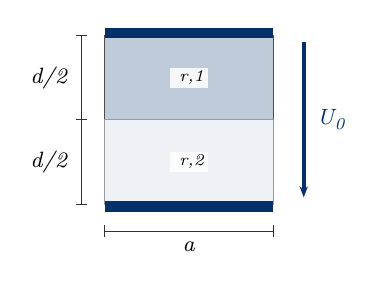
\begin{tikzpicture}[line join=round]
\filldraw[draw=black!70,fill=FAUblue!25] (1.395,-1.930) rectangle (3.536,-0.860);
\filldraw[draw=black!40,fill=Paperblue] (1.395,-3.001) rectangle (3.536,-1.930);
\fill[FAUblue] (1.395,-0.896) rectangle (3.536,-0.760);
\fill[FAUblue] (1.395,-3.101) rectangle (3.536,-2.965);
\node[fill=white,fill opacity=0.85,text opacity=1,inner sep=1pt,font=\footnotesize] at (2.466,-1.395) {\textit{ε\textsubscript{r,1}}};
\node[fill=white,fill opacity=0.85,text opacity=1,inner sep=1pt,font=\footnotesize] at (2.466,-2.466) {\textit{ε\textsubscript{r,2}}};
\draw[black!80] (1.096,-3.001) -- (1.096,-1.930);
\draw[black!80] (1.024,-3.001) -- (1.168,-3.001);
\draw[black!80] (1.024,-1.930) -- (1.168,-1.930);
\node[anchor=east,fill=white,fill opacity=0.85,text opacity=1,inner sep=1pt,font=\footnotesize] at (0.970,-2.466) {\textit{d/2}};
\draw[black!80] (1.096,-1.930) -- (1.096,-0.860);
\draw[black!80] (1.024,-1.930) -- (1.168,-1.930);
\draw[black!80] (1.024,-0.860) -- (1.168,-0.860);
\node[anchor=east,fill=white,fill opacity=0.85,text opacity=1,inner sep=1pt,font=\footnotesize] at (0.970,-1.395) {\textit{d/2}};
\draw[black!80] (1.395,-3.343) -- (3.536,-3.343);
\draw[black!80] (1.395,-3.271) -- (1.395,-3.415);
\draw[black!80] (3.536,-3.271) -- (3.536,-3.415);
\node[fill=white,fill opacity=0.85,text opacity=1,inner sep=1pt,font=\footnotesize] at (2.466,-3.541) {\textit{a}};
\draw[-{Stealth[length=4pt]},FAUblue,line width=1.6pt] (3.921,-0.946) -- (3.921,-2.915);
\node[anchor=west,text=FAUblue,fill=white,fill opacity=0.85,text opacity=1,inner sep=1pt,font=\footnotesize] at (4.047,-1.930) {\textit{U\textsubscript{0}}};
\end{tikzpicture}\par\smallskip{\small\raggedright \textbf{Before the shift: two layers in series.} Dielectric ε\textsubscript{r,1} fills the upper half and ε\textsubscript{r,2} the lower half, each of thickness {\small\ensuremath{\dfrac{{d}}{2}}} over the full plate area \textit{a}\textsuperscript{2}. The voltage \textit{U}\textsubscript{0} points from the top plate to the bottom one.\par}\end{minipage}
\end{center}

\begin{keepsection}
\Needspace{7\baselineskip}
\subsection{8a: Find \textit{D} and \textit{E}}

\Needspace{4\baselineskip}
Try first: use continuity of the normal displacement at the dielectric boundary and add the two half-gap voltage drops.

\nopagebreak[4]{\small\itshape Answers: see “Task 8: Electrostatics” under Answers at the end.}
\end{keepsection}

\begin{keepsection}
\Needspace{7\baselineskip}
\subsection{8b: Equivalent circuit before the shift}

\Needspace{4\baselineskip}
Try first: decide whether the layers lie one after another along the field or side by side across the plate area.

\nopagebreak[4]{\small\itshape Answers: see “Task 8: Electrostatics” under Answers at the end.}
\end{keepsection}

\begin{keepsection}
\Needspace{7\baselineskip}
\subsection{8c: Total capacitance before the shift}

\Needspace{4\baselineskip}
Try first: calculate each layer’s plate capacitance using area \textit{a}\textsuperscript{2} and thickness {\small\ensuremath{\dfrac{{d}}{2}}}, then combine in series.

\nopagebreak[4]{\small\itshape Answers: see “Task 8: Electrostatics” under Answers at the end.}
\end{keepsection}

\begin{keepsection}
\Needspace{6\baselineskip}
\subsection{8d: Surface charge on the lower face of the top plate}

\Needspace{3\baselineskip}
Try first: dot \textit{D} with the outward normal from the metal into the dielectric at that face.

\nopagebreak[4]{\small\itshape Answers: see “Task 8: Electrostatics” under Answers at the end.}

\Needspace{9\baselineskip}
The lower dielectric is now shifted out along +\textit{e}\textsubscript{x} by a distance \textit{x}, with 0 \ensuremath{\leq} \textit{x} \ensuremath{\leq} \textit{a}. Its overlap width is \textit{a}\ensuremath{-}\textit{x}; the exposed gap beneath the upper dielectric is filled with air.

\Needspace{14\baselineskip}
\begin{center}
\begin{minipage}[t]{0.950\linewidth}\centering
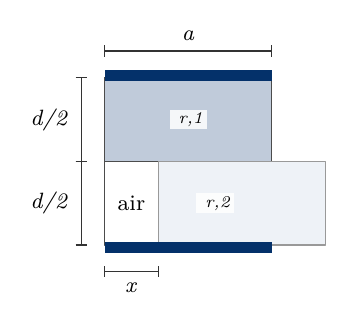
\begin{tikzpicture}[line join=round]
\filldraw[draw=black!70,fill=FAUblue!25] (1.387,-2.024) rectangle (3.510,-0.963);
\filldraw[draw=black!70,fill=white] (1.387,-3.086) rectangle (2.067,-2.024);
\filldraw[draw=black!40,fill=Paperblue] (2.067,-3.086) rectangle (4.190,-2.024);
\fill[FAUblue] (1.387,-0.999) rectangle (3.510,-0.863);
\fill[FAUblue] (1.387,-3.186) rectangle (3.510,-3.050);
\node[fill=white,fill opacity=0.85,text opacity=1,inner sep=1pt,font=\footnotesize] at (2.449,-1.494) {\textit{ε\textsubscript{r,1}}};
\node[fill=white,fill opacity=0.85,text opacity=1,inner sep=1pt,font=\footnotesize] at (1.727,-2.555) {air};
\node[fill=white,fill opacity=0.85,text opacity=1,inner sep=1pt,font=\footnotesize] at (2.789,-2.555) {\textit{ε\textsubscript{r,2}}};
\draw[black!80] (1.387,-3.426) -- (2.067,-3.426);
\draw[black!80] (1.387,-3.354) -- (1.387,-3.498);
\draw[black!80] (2.067,-3.354) -- (2.067,-3.498);
\node[fill=white,fill opacity=0.85,text opacity=1,inner sep=1pt,font=\footnotesize] at (1.727,-3.624) {\textit{x}};
\draw[black!80] (1.387,-0.623) -- (3.510,-0.623);
\draw[black!80] (1.387,-0.551) -- (1.387,-0.695);
\draw[black!80] (3.510,-0.551) -- (3.510,-0.695);
\node[fill=white,fill opacity=0.85,text opacity=1,inner sep=1pt,font=\footnotesize] at (2.449,-0.425) {\textit{a}};
\draw[black!80] (1.090,-3.086) -- (1.090,-2.024);
\draw[black!80] (1.018,-3.086) -- (1.162,-3.086);
\draw[black!80] (1.018,-2.024) -- (1.162,-2.024);
\node[anchor=east,fill=white,fill opacity=0.85,text opacity=1,inner sep=1pt,font=\footnotesize] at (0.964,-2.555) {\textit{d/2}};
\draw[black!80] (1.090,-2.024) -- (1.090,-0.963);
\draw[black!80] (1.018,-2.024) -- (1.162,-2.024);
\draw[black!80] (1.018,-0.963) -- (1.162,-0.963);
\node[anchor=east,fill=white,fill opacity=0.85,text opacity=1,inner sep=1pt,font=\footnotesize] at (0.964,-1.494) {\textit{d/2}};
\end{tikzpicture}\par\smallskip{\small\raggedright \textbf{After the shift by \textit{x}.} The upper layer still covers the whole plate. Below it, a strip of width \textit{x} is air and the rest, width \textit{a} \ensuremath{-} \textit{x}, is still ε\textsubscript{r,2}; the part pushed past the plate edge carries no field.\par}\end{minipage}
\end{center}
\end{keepsection}

\begin{keepsection}
\Needspace{7\baselineskip}
\subsection{8e: Equivalent circuit after the shift}

\Needspace{4\baselineskip}
Try first: identify the full-area layer crossed by every field line, then split the lower half into the two side-by-side regions.

\nopagebreak[4]{\small\itshape Answers: see “Task 8: Electrostatics” under Answers at the end.}
\end{keepsection}

\begin{keepsection}
\Needspace{7\baselineskip}
\subsection{8f: Capacitance as a function of \textit{x}}

\Needspace{4\baselineskip}
Try first: find each lower-region capacitance from its area and thickness, add the parallel branches, then combine that result in series with \textit{C}\textsubscript{1}.

\nopagebreak[4]{\small\itshape Answers: see “Task 8: Electrostatics” under Answers at the end.}
\end{keepsection}

\begin{keepsection}
\Needspace{7\baselineskip}
\subsection{8g: Minimum and maximum capacitance}

\Needspace{4\baselineskip}
Try first: check how the lower parallel capacitance changes with \textit{x}, then use that the series equivalent increases when either component capacitance increases.

\nopagebreak[4]{\small\itshape Answers: see “Task 8: Electrostatics” under Answers at the end.}
\end{keepsection}
\end{keepsection}


\clearpage
\section{Answers}
\begin{keepsection}\subsection{Task 8: Electrostatics}

\begin{workedbox}{8a \ensuremath{\cdot} Fields in the two layers}
\Needspace{11\baselineskip}
\begin{enumerate}
\item \Needspace{6\baselineskip}
With no free charge at the internal interface, the normal component of \textit{D} is the same in both layers. The voltage arrow sets the field downward for positive \textit{U}\textsubscript{0}; denote the downward displacement magnitude by \textit{D}\textsubscript{0}:

\begin{equation*}{D}_{1}\, =\, {D}_{2}\, =\, -{D}_{0}\, {e}_{\mathrm{z}}\end{equation*}
\item \Needspace{5\baselineskip}
In each linear dielectric, \textit{D} = ε\textsubscript{0}ε\textsubscript{r}\textit{E}. The downward potential drop across each thickness {\small\ensuremath{\dfrac{{d}}{2}}} adds to \textit{U}\textsubscript{0}:

\Needspace{4\baselineskip}
\begin{equation*}{U}_{0}\, =\, \dfrac{{D}_{0}}{ε_{0}\, ε_{\mathrm{r},1}}\, \cdot \, \dfrac{{d}}{2}\, +\, \dfrac{{D}_{0}}{ε_{0}\, ε_{\mathrm{r},2}}\, \cdot \, \dfrac{{d}}{2}\end{equation*}

\begin{equation*}{D}_{0}\, =\, \dfrac{2ε_{0}\, ε_{\mathrm{r},1}\, ε_{\mathrm{r},2}\, {U}_{0}}{{d}(ε_{\mathrm{r},1}\, +\, ε_{\mathrm{r},2})}\end{equation*}
\item \Needspace{4\baselineskip}
Apply the constitutive relation separately to each layer:

\Needspace{4\baselineskip}
\begin{equation*}{D}\, =\, -\dfrac{2ε_{0}\, ε_{\mathrm{r},1}\, ε_{\mathrm{r},2}\, {U}_{0}}{{d}(ε_{\mathrm{r},1}\, +\, ε_{\mathrm{r},2})}\, {e}_{\mathrm{z}}\end{equation*}

\Needspace{5\baselineskip}
\begin{equation*}{E}_{1}\, =\, -\dfrac{2ε_{\mathrm{r},2}\, {U}_{0}}{{d}(ε_{\mathrm{r},1}\, +\, ε_{\mathrm{r},2})}\, {e}_{\mathrm{z}},\quad \, \quad \, {E}_{2}\, =\, -\dfrac{2ε_{\mathrm{r},1}\, {U}_{0}}{{d}(ε_{\mathrm{r},1}\, +\, ε_{\mathrm{r},2})}\, {e}_{\mathrm{z}}\end{equation*}

For negative \textit{U}\textsubscript{0}, the vectors reverse. \textbf{Check:} substituting the two field magnitudes into the half-gap drops gives exactly \textit{U}\textsubscript{0}.
\end{enumerate}
\end{workedbox}

\end{keepsection}
\begin{keepsection}\subsection{Task 8: Electrostatics}

\begin{workedbox}{8b \ensuremath{\cdot} Series connection}
\Needspace{9\baselineskip}
\begin{enumerate}
\item \Needspace{6\baselineskip}
Every field line crosses dielectric 1 and then dielectric 2. The same free charge magnitude sits on each plate, while the voltage divides between the layers, so the capacitors are in series:

\Needspace{8\baselineskip}
\begin{equation*}{C}_{1}\, \text{in}\, \text{series}\, \text{with}\, {C}_{2}\end{equation*}

\Needspace{14\baselineskip}
\begin{center}
\begin{minipage}[t]{0.950\linewidth}\centering
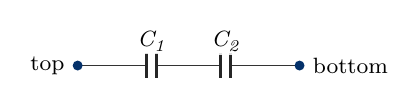
\begin{tikzpicture}[line join=round]
\draw[black!80] (1.136,-0.995) -- (3.954,-0.995);
\fill[white] (2.003,-0.833) rectangle (2.147,-1.157);
\draw[black!85,line width=1pt] (2.012,-0.833) -- (2.012,-1.157);
\draw[black!85,line width=1pt] (2.138,-0.833) -- (2.138,-1.157);
\fill[white] (2.943,-0.833) rectangle (3.087,-1.157);
\draw[black!85,line width=1pt] (2.952,-0.833) -- (2.952,-1.157);
\draw[black!85,line width=1pt] (3.078,-0.833) -- (3.078,-1.157);
\fill[FAUblue] (1.136,-0.995) circle (0.063);
\fill[FAUblue] (3.954,-0.995) circle (0.063);
\node[fill=white,fill opacity=0.85,text opacity=1,inner sep=1pt,font=\footnotesize] at (2.075,-0.685) {\textit{C\textsubscript{1}}};
\node[fill=white,fill opacity=0.85,text opacity=1,inner sep=1pt,font=\footnotesize] at (3.015,-0.685) {\textit{C\textsubscript{2}}};
\node[anchor=east,fill=white,fill opacity=0.85,text opacity=1,inner sep=1pt,font=\footnotesize] at (1.010,-0.995) {top};
\node[anchor=west,fill=white,fill opacity=0.85,text opacity=1,inner sep=1pt,font=\footnotesize] at (4.080,-0.995) {bottom};
\end{tikzpicture}\par\smallskip{\small\raggedright \textbf{Series.} One path from the top plate to the bottom plate through both layers: the same charge on each, the voltage shared.\par}\end{minipage}
\end{center}
\item The interface has no free surface charge, so the normal displacement (and therefore the series charge) is common to both. \textbf{Check:} a parallel model would incorrectly assign the full plate voltage to each half-thickness layer.
\end{enumerate}
\end{workedbox}

\end{keepsection}
\begin{keepsection}\subsection{Task 8: Electrostatics}

\begin{workedbox}{8c \ensuremath{\cdot} Series capacitance}
\Needspace{6\baselineskip}
\begin{enumerate}
\item \Needspace{4\baselineskip}
For a parallel-plate layer, \textit{C} = {\small\ensuremath{\dfrac{ε{A}}{{t}}}}. Each layer has area \textit{a}\textsuperscript{2} and thickness {\small\ensuremath{\dfrac{{d}}{2}}}:

\begin{equation*}{C}_{1}\, =\, \dfrac{2ε_{0}\, ε_{\mathrm{r},1}\, {a}^{2}}{{d}},\quad \, \quad \, {C}_{2}\, =\, \dfrac{2ε_{0}\, ε_{\mathrm{r},2}\, {a}^{2}}{{d}}\end{equation*}
\item \Needspace{4\baselineskip}
Series capacitances add by reciprocals:

\Needspace{4\baselineskip}
\begin{equation*}\dfrac{1}{{C}}\, =\, \dfrac{1}{{C}_{1}}\, +\, \dfrac{1}{{C}_{2}}\end{equation*}

\Needspace{4\baselineskip}
\begin{equation*}{C}\, =\, \dfrac{2ε_{0}\, {a}^{2}\, ε_{\mathrm{r},1}\, ε_{\mathrm{r},2}}{{d}(ε_{\mathrm{r},1}\, +\, ε_{\mathrm{r},2})}\end{equation*}

\textbf{Check:} this is smaller than either layer capacitance, as a series equivalent must be.
\end{enumerate}
\end{workedbox}

\end{keepsection}
\begin{keepsection}\subsection{Task 8: Electrostatics}

\begin{workedbox}{8d \ensuremath{\cdot} Free surface charge density}
\Needspace{7\baselineskip}
\begin{enumerate}
\item \Needspace{5\baselineskip}
The bottom face of the top plate points outward from the conductor in the \ensuremath{-}\textit{e}\textsubscript{z} direction. The free charge density on a conductor surface is \textit{D} \ensuremath{\cdot} \textit{n} just outside the metal:

\begin{equation*}σ_{0}\, =\, {D}\, \cdot \, (-{e}_{\mathrm{z}})\end{equation*}
\item \Needspace{4\baselineskip}
Since \textit{D} also points downward for positive \textit{U}\textsubscript{0}, the dot product is positive:

\Needspace{4\baselineskip}
\begin{equation*}σ_{0}\, =\, \dfrac{2ε_{0}\, ε_{\mathrm{r},1}\, ε_{\mathrm{r},2}\, {U}_{0}}{{d}(ε_{\mathrm{r},1}\, +\, ε_{\mathrm{r},2})}\end{equation*}

The units are C/m². Reversing the applied voltage reverses the surface-charge sign.
\end{enumerate}
\end{workedbox}

\end{keepsection}
\begin{keepsection}\subsection{Task 8: Electrostatics}

\begin{workedbox}{8e \ensuremath{\cdot} Series and parallel sections}
\Needspace{8\baselineskip}
\begin{enumerate}
\item \Needspace{6\baselineskip}
All paths pass through dielectric 1 across the full area \textit{a}\textsuperscript{2}. In the lower half, some area \textit{a}(\textit{a}\ensuremath{-}\textit{x}) contains dielectric 2 and the remaining area \textit{a x} contains air. Those lower branches share the same voltage:

\Needspace{8\baselineskip}
\begin{equation*}{C}_{1}\, \text{in}\, \text{series}\, \text{with}\, ({C}_{2}\, ∥\, {C}_{\mathrm{L}})\end{equation*}

\Needspace{14\baselineskip}
\begin{center}
\begin{minipage}[t]{0.950\linewidth}\centering
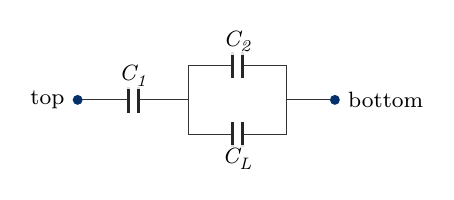
\begin{tikzpicture}[line join=round]
\draw[black!80] (1.094,-1.183) -- (2.507,-1.183);
\draw[black!80] (2.507,-0.741) -- (2.507,-1.624);
\draw[black!80] (2.507,-0.741) -- (3.743,-0.741);
\draw[black!80] (2.507,-1.624) -- (3.743,-1.624);
\draw[black!80] (3.743,-0.741) -- (3.743,-1.624);
\draw[black!80] (3.743,-1.183) -- (4.361,-1.183);
\fill[white] (1.729,-1.021) rectangle (1.873,-1.345);
\draw[black!85,line width=1pt] (1.738,-1.021) -- (1.738,-1.345);
\draw[black!85,line width=1pt] (1.864,-1.021) -- (1.864,-1.345);
\fill[white] (3.053,-0.579) rectangle (3.197,-0.903);
\draw[black!85,line width=1pt] (3.062,-0.579) -- (3.062,-0.903);
\draw[black!85,line width=1pt] (3.188,-0.579) -- (3.188,-0.903);
\fill[white] (3.053,-1.462) rectangle (3.197,-1.786);
\draw[black!85,line width=1pt] (3.062,-1.462) -- (3.062,-1.786);
\draw[black!85,line width=1pt] (3.188,-1.462) -- (3.188,-1.786);
\fill[FAUblue] (1.094,-1.183) circle (0.063);
\fill[FAUblue] (4.361,-1.183) circle (0.063);
\node[fill=white,fill opacity=0.85,text opacity=1,inner sep=1pt,font=\footnotesize] at (1.801,-0.879) {\textit{C\textsubscript{1}}};
\node[fill=white,fill opacity=0.85,text opacity=1,inner sep=1pt,font=\footnotesize] at (3.125,-0.437) {\textit{C\textsubscript{2}}};
\node[fill=white,fill opacity=0.85,text opacity=1,inner sep=1pt,font=\footnotesize] at (3.125,-1.928) {\textit{C\textsubscript{L}}};
\node[anchor=east,fill=white,fill opacity=0.85,text opacity=1,inner sep=1pt,font=\footnotesize] at (0.968,-1.183) {top};
\node[anchor=west,fill=white,fill opacity=0.85,text opacity=1,inner sep=1pt,font=\footnotesize] at (4.487,-1.183) {bottom};
\end{tikzpicture}\par\smallskip{\small\raggedright \textbf{Series, then parallel.} Every path crosses C\textsubscript{1}; below it the path splits between the ε\textsubscript{r,2} part (C\textsubscript{2}) and the air strip (C\textsubscript{L}), which share one voltage.\par}\end{minipage}
\end{center}
\item Thus \textit{C}\textsubscript{2} and \textit{C}\textsubscript{L} are in parallel with one another, and their equivalent is in series with \textit{C}\textsubscript{1}. \textbf{Check:} at \textit{x} = 0 the air branch has zero area; at \textit{x} = \textit{a} the lower dielectric branch has zero area.
\end{enumerate}
\end{workedbox}

\end{keepsection}
\begin{keepsection}\subsection{Task 8: Electrostatics}

\begin{workedbox}{8f \ensuremath{\cdot} Capacitance after displacement}
\Needspace{8\baselineskip}
\begin{enumerate}
\item \Needspace{4\baselineskip}
The upper layer keeps area \textit{a}\textsuperscript{2} and thickness {\small\ensuremath{\dfrac{{d}}{2}}}. The two lower branches each have thickness {\small\ensuremath{\dfrac{{d}}{2}}}:

\Needspace{4\baselineskip}
\begin{equation*}{C}_{1}\, =\, \dfrac{2ε_{0}\, ε_{\mathrm{r},1}\, {a}^{2}}{{d}}\end{equation*}

\begin{equation*}{C}_{2}({x})\, =\, \dfrac{2ε_{0}\, ε_{\mathrm{r},2}\, {a}({a}\, -\, {x})}{{d}},\quad \, \quad \, {C}_{\mathrm{L}}({x})\, =\, \dfrac{2ε_{0}\, {a}\, {x}}{{d}}\end{equation*}
\item \Needspace{4\baselineskip}
Add the parallel pair and then use the series formula:

\Needspace{4\baselineskip}
\begin{equation*}{C}_{\mathrm{p}}({x})\, =\, {C}_{2}({x})\, +\, {C}_{\mathrm{L}}({x})\, =\, \dfrac{2ε_{0}\, {a}}{{d}}[ε_{\mathrm{r},2}\, {a}\, +\, (1\, -\, ε_{\mathrm{r},2}){x}]\end{equation*}

\Needspace{4\baselineskip}
\begin{equation*}{C}({x})\, =\, \dfrac{{C}_{1}\, {C}_{\mathrm{p}}({x})}{{C}_{1}\, +\, {C}_{\mathrm{p}}({x})}\end{equation*}

\Needspace{5\baselineskip}
\begin{equation*}{C}({x})\, =\, \dfrac{2ε_{0}\, {a}}{{d}}\, \cdot \, \dfrac{ε_{\mathrm{r},1}\, {a}[ε_{\mathrm{r},2}\, {a}\, +\, (1\, -\, ε_{\mathrm{r},2}){x}]}{ε_{\mathrm{r},1}\, {a}\, +\, ε_{\mathrm{r},2}\, {a}\, +\, (1\, -\, ε_{\mathrm{r},2}){x}}\end{equation*}

\textbf{Endpoint checks:} \textit{C}(0) matches 8c, while \textit{C}(\textit{a}) is the series combination of the upper dielectric and an air layer of thickness {\small\ensuremath{\dfrac{{d}}{2}}}.
\end{enumerate}
\end{workedbox}

\end{keepsection}
\begin{keepsection}\subsection{Task 8: Electrostatics}

\begin{workedbox}{8g \ensuremath{\cdot} Locate the extrema}
\Needspace{10\baselineskip}
\begin{enumerate}
\item \Needspace{4\baselineskip}
The lower equivalent is linear in \textit{x}:

\Needspace{5\baselineskip}
\begin{equation*}{C}_{\mathrm{p}}({x})\, =\, \dfrac{2ε_{0}\, {a}}{{d}}[ε_{\mathrm{r},2}\, {a}\, +\, (1\, -\, ε_{\mathrm{r},2}){x}]\end{equation*}

Because ε\textsubscript{r,2} is much greater than 1, its slope is negative. The series equivalent {\small\ensuremath{\dfrac{{C}_{1}{C}_{\mathrm{p}}}{{C}_{1}+{C}_{\mathrm{p}}}}} increases monotonically with \textit{C}\textsubscript{p}.
\item \Needspace{4\baselineskip}
Therefore the total capacitance decreases throughout 0 \ensuremath{\leq} \textit{x} \ensuremath{\leq} \textit{a}:

\Needspace{5\baselineskip}
\begin{equation*}\text{maximum}\, \text{at}\, {x}\, =\, 0,\quad \, \quad \, \text{minimum}\, \text{at}\, {x}\, =\, {a}\end{equation*}

\Needspace{9\baselineskip}
If ε\textsubscript{r,2} were exactly 1, the lower region would be air everywhere and the capacitance would be constant; the sheet specifies ε\textsubscript{r,2} much greater than 1, excluding that degenerate case.

\Needspace{14\baselineskip}
\begin{center}
\begin{minipage}[t]{0.950\linewidth}\centering
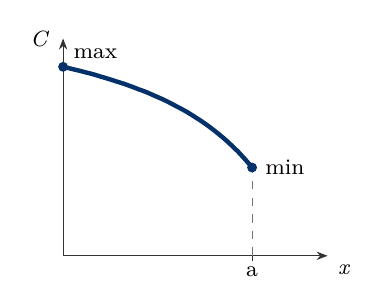
\begin{tikzpicture}[line join=round]
\draw[-{Stealth[length=4pt]},black!80] (1.152,-3.312) -- (4.512,-3.312);
\node[anchor=west,fill=white,fill opacity=0.85,text opacity=1,inner sep=1pt,font=\footnotesize] at (4.602,-3.492) {\textit{x}};
\draw[-{Stealth[length=4pt]},black!80] (1.152,-3.312) -- (1.152,-0.552);
\node[anchor=east,fill=white,fill opacity=0.85,text opacity=1,inner sep=1pt,font=\footnotesize] at (1.026,-0.552) {\textit{C}};
\draw[black!80] (3.552,-3.240) -- (3.552,-3.384);
\node[fill=white,fill opacity=0.85,text opacity=1,inner sep=1pt,font=\footnotesize] at (3.552,-3.510) {a};
\draw[black!55,dashed] (3.552,-3.312) -- (3.552,-2.191);
\draw[FAUblue,line width=1.6pt] (1.152,-0.912) -- (1.212,-0.926) -- (1.272,-0.941) -- (1.332,-0.955) -- (1.392,-0.970) -- (1.452,-0.986) -- (1.512,-1.001) -- (1.572,-1.018) -- (1.632,-1.037) -- (1.692,-1.054) -- (1.752,-1.073) -- (1.812,-1.092) -- (1.872,-1.111) -- (1.932,-1.130) -- (1.992,-1.152) -- (2.052,-1.174) -- (2.112,-1.198) -- (2.172,-1.219) -- (2.232,-1.243) -- (2.292,-1.270) -- (2.352,-1.296) -- (2.412,-1.322) -- (2.472,-1.351) -- (2.532,-1.382) -- (2.592,-1.414) -- (2.652,-1.445) -- (2.712,-1.478) -- (2.772,-1.514) -- (2.832,-1.553) -- (2.892,-1.591) -- (2.952,-1.632) -- (3.012,-1.675) -- (3.072,-1.721) -- (3.132,-1.769) -- (3.192,-1.819) -- (3.252,-1.872) -- (3.312,-1.930) -- (3.372,-1.987) -- (3.432,-2.052) -- (3.492,-2.119) -- (3.552,-2.191);
\fill[FAUblue] (1.152,-0.912) circle (0.063);
\fill[FAUblue] (3.552,-2.191) circle (0.063);
\node[anchor=west,fill=white,fill opacity=0.85,text opacity=1,inner sep=1pt,font=\footnotesize] at (1.242,-0.750) {max};
\node[anchor=west,fill=white,fill opacity=0.85,text opacity=1,inner sep=1pt,font=\footnotesize] at (3.678,-2.191) {min};
\end{tikzpicture}\par\smallskip{\small\raggedright \textbf{Capacitance falls all the way.} Drawn for ε\textsubscript{r,1} = 2 and ε\textsubscript{r,2} = 5. As the strip of air widens, \textit{C}(\textit{x}) only decreases, so the extremes sit at the two ends of the range.\par}\end{minipage}
\end{center}
\end{enumerate}
\end{workedbox}

\end{keepsection}

\vfill{\small Personal worked-solution guide based on the supplied EE1 Tutorial Task sheet, written in my own words; no tutorial text or figures are reproduced. Not an official FAU publication; check course details against current material. Made by \textbf{Thanate Amornjiraporn (Focus)}.}

\end{document}
